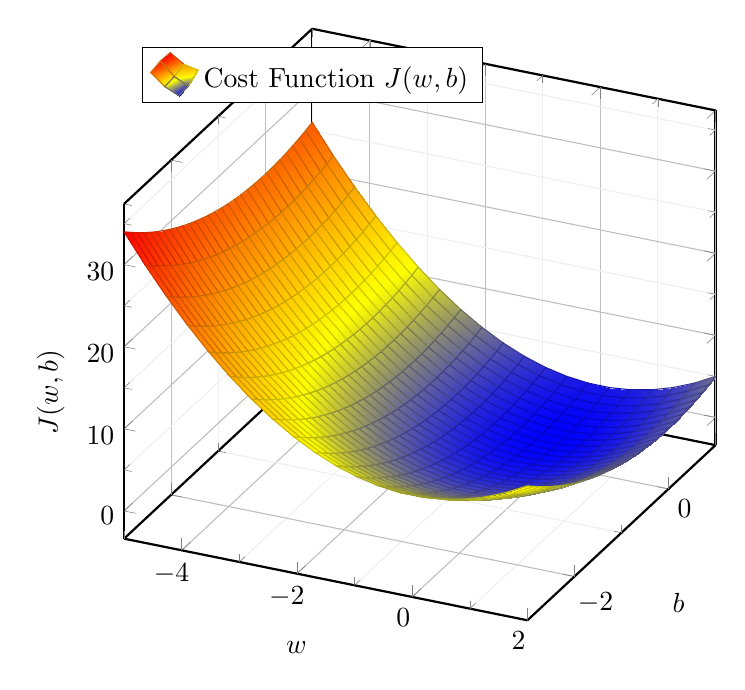
\begin{tikzpicture}
    \begin{axis}[
        width = 0.75\textwidth,
        height = 0.75\textwidth,
        grid = both,
        minor tick num = 1,
        major grid style = {lightgray},
        minor grid style = {lightgray!25},
        xlabel = {$w$},
        ylabel = {$b$},
        zlabel = {$J(w,b)$},
        legend cell align = {left},
        legend pos = north west,
        axis line style = {thick},
        % colormap/viridis
    ]
    
    \addplot3 [
        domain=-5:2,
        domain y = -3:1,
        samples = 20,
        samples y = 30,
        surf,
        shader=faceted interp] {x^2 + y^2};
     
    % Add legend
    \addlegendentry{Cost Function $J(w, b)$}
     
    \end{axis}
    \end{tikzpicture}